\chapter{A Detour to Differential Geometry}
\label{cha:a_small_detour_to_differential_geometry}

\begin{enumerate}
    \makethislistcompact
    \item Manifolds
    \item Morphism of manifolds -  Smooth mappings etc.
    \item Types of submanifolds - Immersion, Embedding etc.
    \item Tangent Spaces
    \item Differential forms
\end{enumerate}

\begin{insight} % smooth manifold vs smooth varieties
    Let 
    \begin{align}
        f: \GL_n(\RR) \to \GL_n(\RR)
    \end{align}
    be a polynomial. This will always be smooth as a manifold. So, in algebraic geometry, the term `smoothness' is reserved for something stronger.
\end{insight}

\section{Tangent Spaces}
\label{sec:tangent_spaces}

\emph{Reference for this section is \cite{brocker1982introduction}.}

Let $M$ and $N$ be differentiable manifolds. Let $f: M\to N$. On the set of all differentiable functions defined at a neighbourhood around a point $p\in M$
\begin{align}
    \{f\ |\ f: U\to N, \quad U\subset M \text{ is a neighbourhood of $p\in M$}\}
\end{align}
we define the equivalence relation
\begin{align}
    f \sim g \iff \exists V\subset M \text{ such that } f|_V = g|_V.
\end{align}
The equivalence classes are called \emph{germs} at the point $p\in M$. We denoted the germs as $\bar f: (M,n)\to (N,q)$. A \emph{function germ} is an equivalence class for maps $(M,p)\to \RR$. The set of all function germ at $p\in M$ is denoted by $\mathcal E(p)$. If we defined addition and multiplication on $\germs(p)$ by the usual operations on their representatives, then $\germs (p)$ acquires the structure of a real algebra.
\begin{insight}
    We need to check if the multiplication and addition are well defined. Lets do it for multiplication.That is, given $\bar f_1 = \bar f_2$ and $\bar g_1 = \bar g_2$, do we have $\bar f_1 \bar g_1 = \bar f_2 \bar g_2$, or $\overline{f_1 g_1}=\overline{f_2 g_2}$? We need to find some $U\in M$ such that $f_1g_1=f_2g_2$ on $U$. Since, $f_1$ and $f_2$ agree on some $V_f\in M$ and $g_1$ and $g_2$ agree on some $V_g\in M$, the products $f_1 g_1$ and $f_2 g_2$ agree on $U=V_f\cap V_g$. Therefore, $\overline{f_1 g_1} = \overline{f_2 g_2}$ and the multiplication is well defined. 
\end{insight}
%The set of all germs at a point form the 

Any differentiable germ $\bar f: (M,p)\to (N,q)$ induces a map real algebra homomorphism $f^*: \germs(q)\to\germs(p)$ via composition $\bar\phi \mapsto f^*(\bar\phi)=\bar\phi\cdot \bar f$. The ($^*$) is thus a \emph{contravariant functor}.

\begin{center}
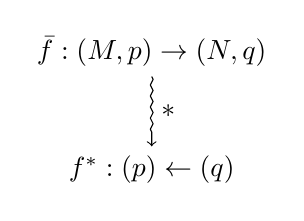
\begin{tikzpicture}[ node distance=1.5cm,
    functor/.style= {
        ->, 
        line join=round,
        decorate, 
        decoration={
            zigzag,
            segment length=4,
            amplitude=.5,
            post=lineto,
            post length=5pt
    } } ]
    \node (bar f) {$\bar f: (M,p)\to (N,q)$};
    \node (f*) [below of=bar f] {$f^*: \germs(p)\gets \germs(q)$} ;
    \draw [functor] (bar f) -- (f*)node[midway, right] {$*$};
\end{tikzpicture}
\end{center}

\subsection{Algebraist's definition}
\label{sub:algebraist_s_definition}

\begin{center}
\begin{tikzcd}[column sep=8pt]
    \bar f: (M,p) \arrow[rr, ""{name=U1, below}, "f" above] {} & & (N,q) \\
    f^*: \germs(p) \arrow[rr, phantom, ""{name=U2, below}] {} & \arrow[rightsquigarrow, from=U1, "*", end anchor={[yshift=3pt]}]& \arrow[ll] \germs(q) \\
    T_p f: T_p M \arrow[rr, ""{name=U3, below}] {} & \arrow[rightsquigarrow, from=U2, "T",end anchor={[yshift=3pt]}] & T_q N 
\end{tikzcd}

\end{center}

\subsection{Physicist's definition}
\label{sub:physicist_s_definition}
\subsection{Geometer's definition}
\label{sub:geometer_s_definition}


